\section{Hitelesítési feladatok}
integritásvédelem, hitelesítés, letagadhatatlanság

\subsection{Hash függvények}
\textbf{Elvárt tulajdonságok:}
	\begin{itemize}
		\item \textbf{(Erős) ütközés-ellenállóság}: Egy h hash függény erősen ütközés-ellenálló, ha nehéz feladat két olyan küönböző ősképtérbeli $x_1 \neq x_2$ elemet találni, melynek hash értéke megegezik x hash értékével, azaz $ h(x_1) = h(x_2)$-et nehéz találni
		\item \textbf{Egyirányúság:} Egy h hash függvény egyirányú, ha bármely y képtérbeli elemhez, melynek ősképe a priori nem ismer, nehéz feladat olyan ősképtérbeli x elemet találni, melynek hash értéke pontosan y, azaz h(x) = y.
	\end{itemize}

\textbf{A születésnapi paradoxon:}

$Szamolas \ldots$ 23 véletlenül választott ember közül, 0.5 valószínűséggel van ugyanazon a napon születésnap. 41 között már 0.9 valószínűséggel $\Longrightarrow$ Ez igaz a hash függvényekre is, ezért a hash függvény kimenetének mérete maw már legalább $n = 128 bit$

\subsection{Iteratív hash függvények}

\begin{center}
	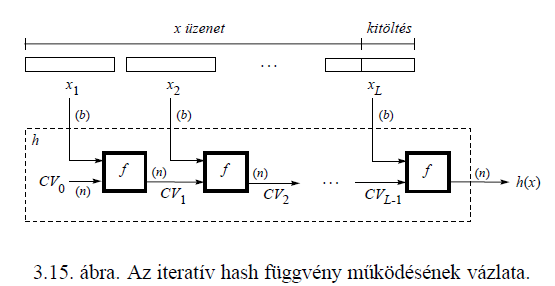
\includegraphics[scale=0.7]{img/ITHASH}
\end{center}

Ha a bemenet nem egész számú többszöröse b-nek, akkor a bemeneti üzenetet ki kell egészíteni pl: Az üzenet hosszával.

\textbf{PL:}
	\begin{itemize}
		\item MD5 \ - 128 bit kimenet
		\item SHA-1 \ - 160 bit kimenet
	\end{itemize}
	Bemenet mindkét esetben 512 bites blokkokban kerül feldolgozásra

\subsection{Üzenethitelesítő kódok (Integrity megvalósítása) }
Message Authentication Code - MAC. Hasonlít a kriptográfiai ellenörzőösszegre .\\[-2pt]

\textbf{Különbség} üzenethitelesítő és hibadetektáló kód(CRC) között:

\forceindent Hibadetektáló - Csak a zajos csatornán bekövetkezett véletlen hibák detektálására alkalmasak, és nem képesek egy rosszindalatú támadó által végrehajtott szándékos módosítások detektálására.( Támadó módosítás után az ellenörző összeget is ujraszámíthatja)

\forceindent Üzenethitelesítő - Nem csak a véletlen hibákat, hanem a rosszindulatú módosításokat is képesek detektálni.\textbf{ Az üzenethitelesítő kód, nem csak az üzenettül, hanem a küldő és a vevő által megosztott titkos információtól( akár kulcs) is függ}

\subsection{Digitális aláírás}

Üzenethitelesítő kódnál a kulcsot csak a vevő ismeri, így egy harmadik felet nem tud meggyőzni hogy a vett üzenet a küldőtől származik.

\begin{enumerate}
	\item Küldő oldalon, X üzenet. Aláírás = $D_A(X)$
	\item Vevő oldalon ellenörzés. $ X = E_A(D_A(X))$
\end{enumerate}
%TODO Példát írni rá
